\documentclass{beamer}

%% figures path
\usepackage[]{graphicx}
\graphicspath{{figure/}}

%% font
\usepackage{avant}
\renewcommand*\familydefault{\sfdefault} %% Only if the base font of the document is to be sans serif
\usepackage[T1]{fontenc}

% colors
\usepackage{xcolor}  % Coloured text etc.
\definecolor{gr}{HTML}{4bc134}
\definecolor{gr2}{HTML}{004d00}
\definecolor{bl}{HTML}{3383c1}

%% tikz
\usepackage{tikz}
\usetikzlibrary{positioning, decorations.pathreplacing, calc, fit, shapes, backgrounds}
\usepackage{fix-cm}
\usepackage{amsfonts}
\usepackage{xifthen}

%% title page
\author{Heidi Seibold}
\title{
\includegraphics[width=0.4\textwidth]{OpenMLLogo}}
\date{Lunch time lecture, October 2017}

\begin{document}


\thispagestyle{empty}
\begin{frame}
\transsplithorizontalout
\titlepage
\end{frame}

\begin{frame}[fragile]{OpenML.org}
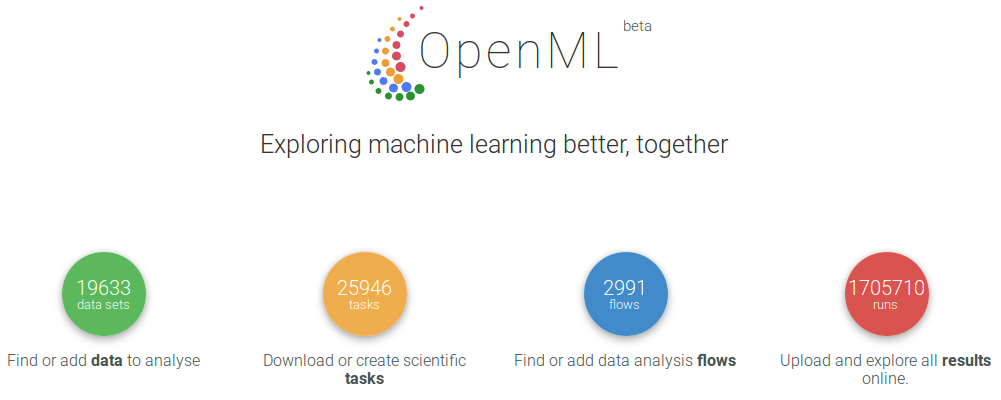
\includegraphics[width = \textwidth]{screenshot}
\end{frame}

\begin{frame}[fragile]{Machine Learning}
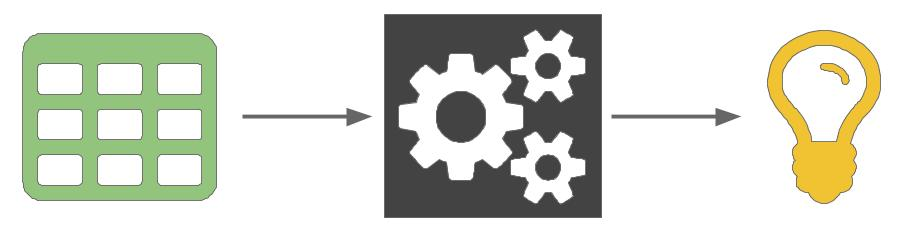
\includegraphics[width = \textwidth]{ML}
\end{frame}

\begin{frame}[fragile]{}
\large 
\begin{center}
Data analysis and machine learning are important in research 
fields where data are collected.\\[2em]

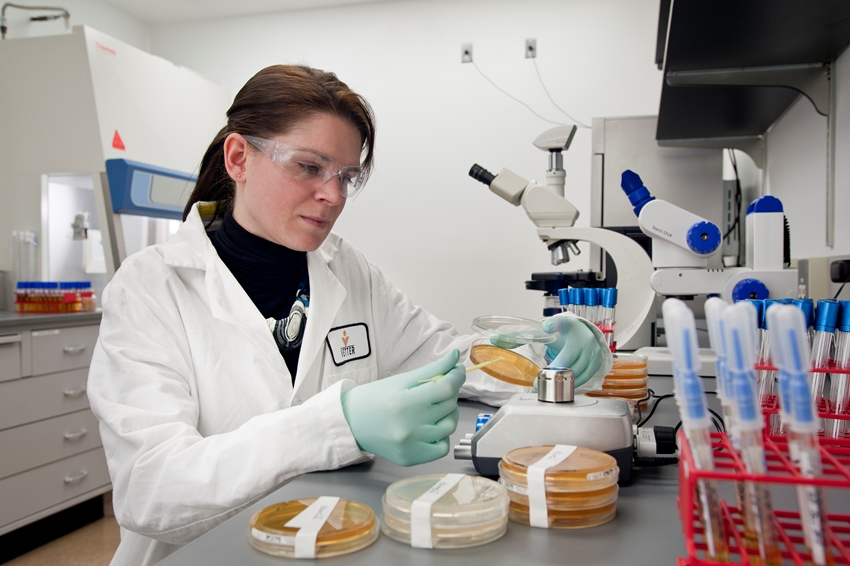
\includegraphics[width = 0.3\textwidth]{lab}
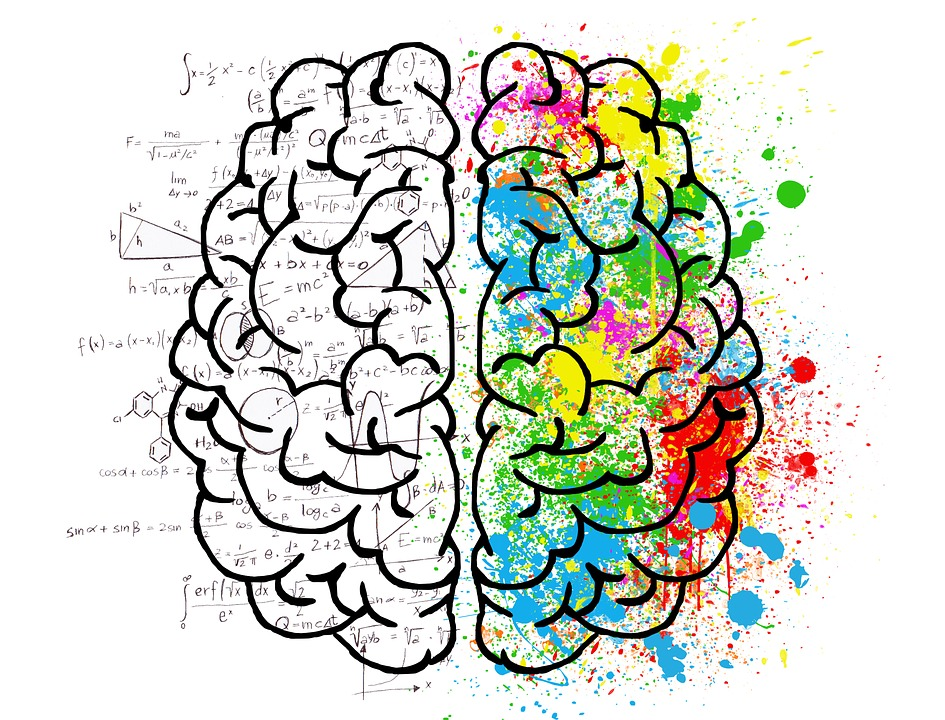
\includegraphics[width = 0.3\textwidth]{psy}

\includegraphics[width = 0.3\textwidth]{wifi}
\end{center}
\end{frame}

\begin{frame}[fragile]{}
\large 
\begin{center}
But many reasearchers need help with this.\\

\includegraphics[width = 0.3\textwidth]{confused}\\
OpenML can be a way to ask machine learners all over the world for help.
\end{center}
\end{frame}

\begin{frame}[fragile]{OpenML machine learner workflow}
\begin{center}
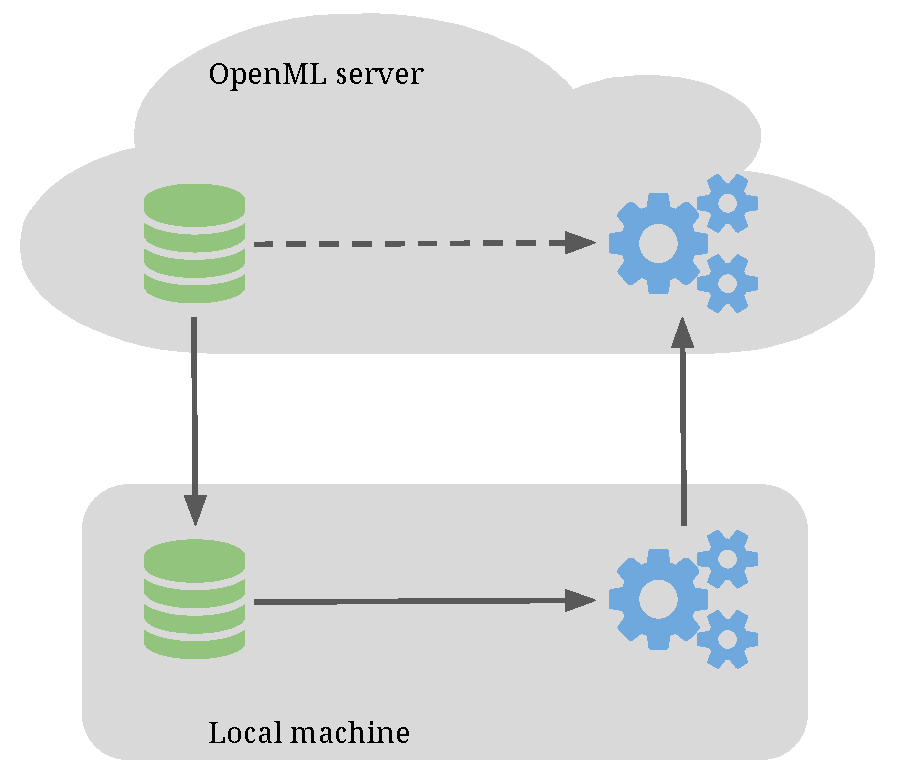
\includegraphics[width = 0.6\textwidth]{wf}
\end{center}
\end{frame}

\begin{frame}[fragile]{One question, many answers}
\begin{center}
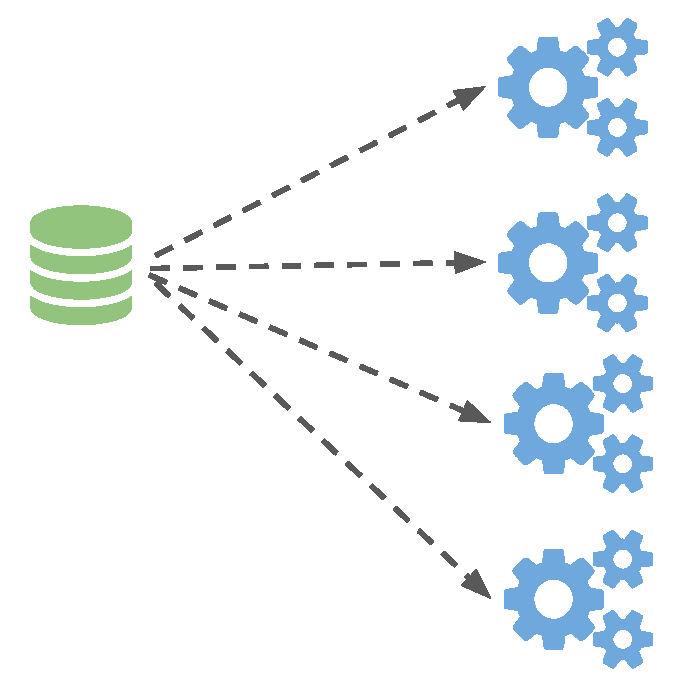
\includegraphics[width = 0.6\textwidth]{wf_ds}\\[2em]
\large $\Rightarrow$ pick the best!
\end{center}
\end{frame}


\begin{frame}[fragile]{Upload a data set}
\begin{center}

\includegraphics[width = 0.5\textwidth]{add}
\end{center}
\end{frame}

\begin{frame}[fragile]{Upload a data set}
\begin{center}
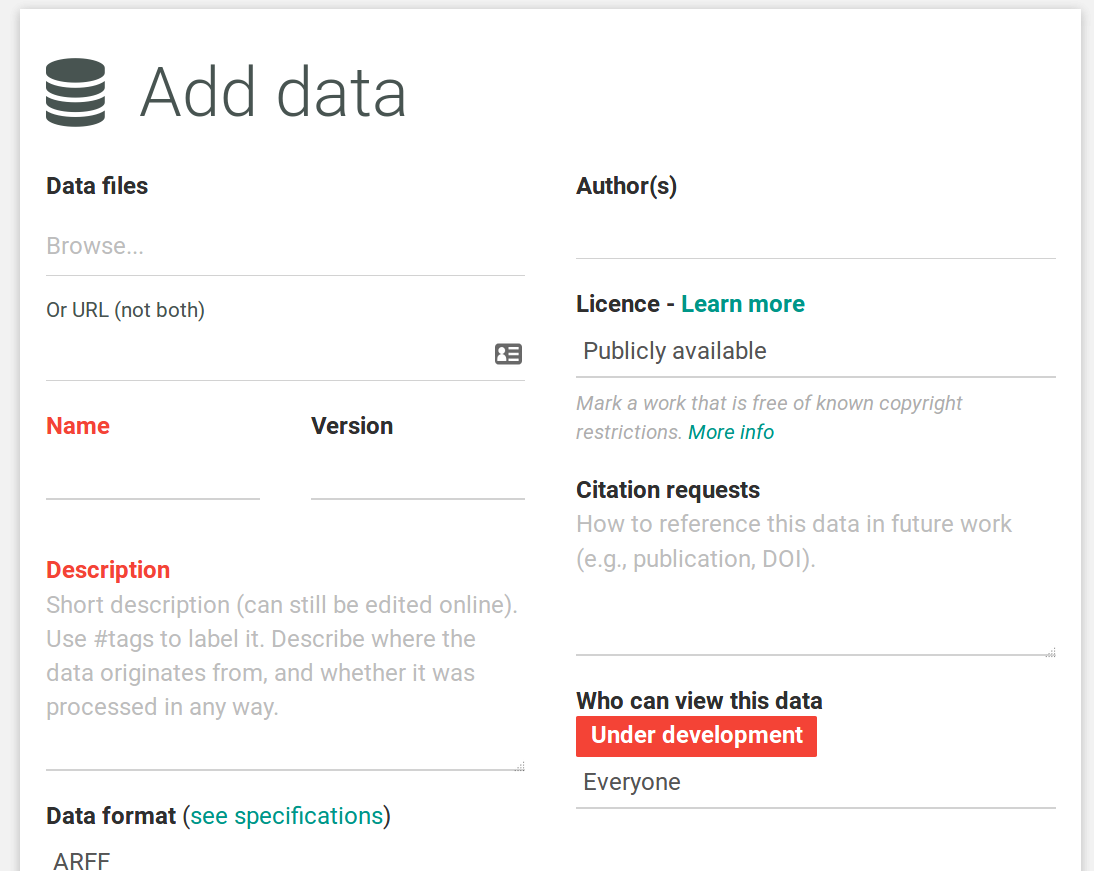
\includegraphics[width = 0.8\textwidth]{add_data}
\end{center}
\end{frame}

\begin{frame}[fragile]{Create a task}
\begin{center}
task = the question = prediction problem\\[2em]
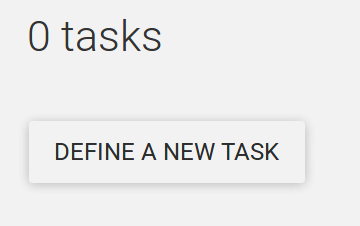
\includegraphics[width = 0.6\textwidth]{add_task}
\end{center}
\end{frame}


\begin{frame}[fragile]{Create a task}
\begin{center}
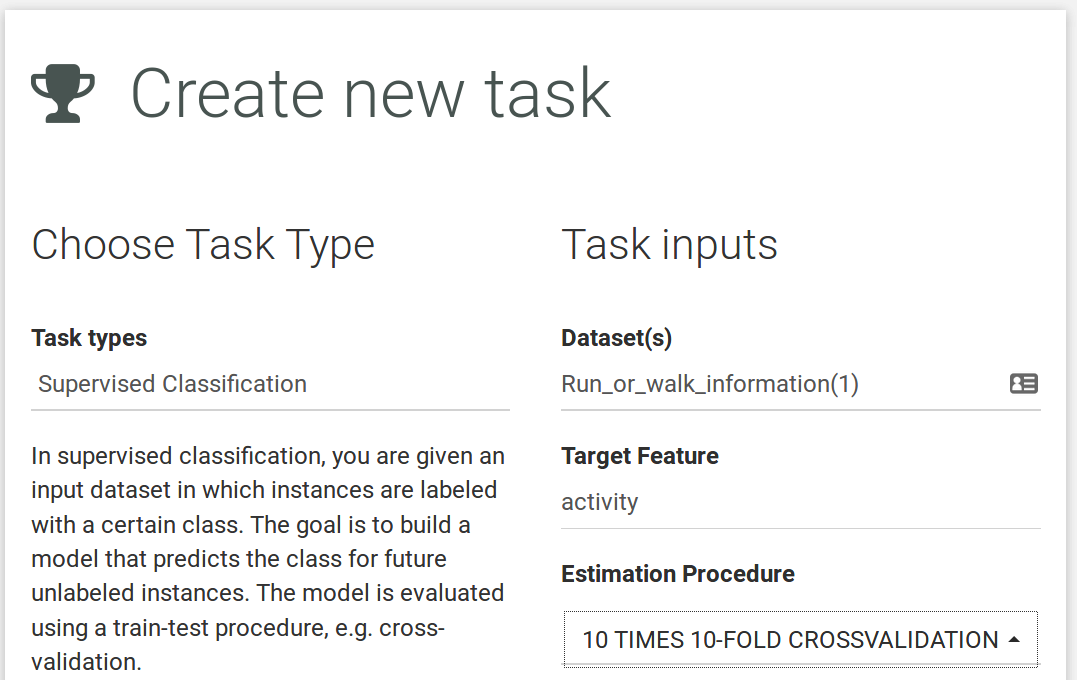
\includegraphics[width = 0.8\textwidth]{add_task2}
\end{center}
\end{frame}

\begin{frame}[fragile]{}
\begin{center}
\Large Now is your turn. Try OpenML and let us know what you think!\\[2em]
\url{https://github.com/openml/OpenML/issues}
\end{center}
\end{frame}


\begin{frame}[fragile]{Want to get involved?}
Start by participating in hacktoberfest!
\begin{center}
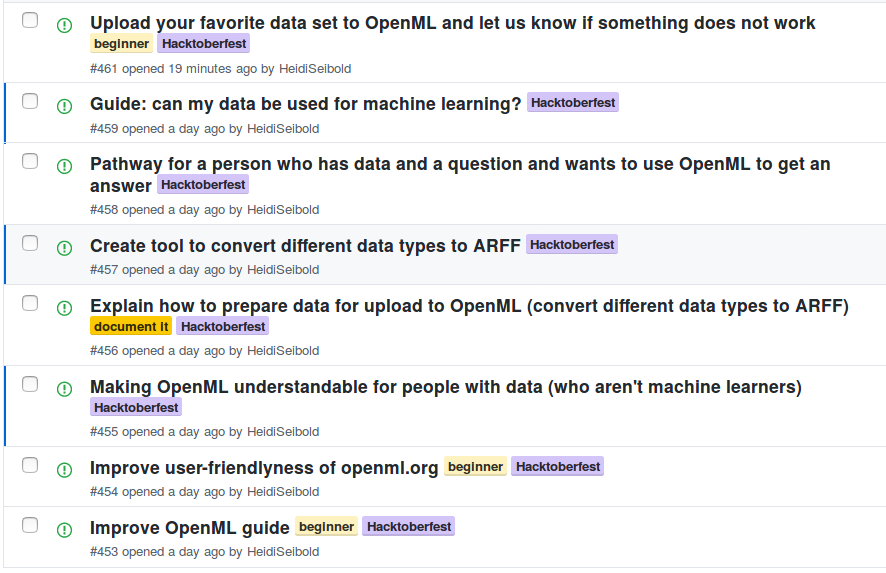
\includegraphics[width = 0.8\textwidth]{issues}\\
\url{https://github.com/openml/OpenML/issues}
\end{center}
\end{frame}

\begin{frame}[fragile]{}
\begin{center}
\Large
Questions?\\
Comments?\\[3em]
\end{center}
Contact:\\
\begin{description}
 \item[Heidi:] \url{heidi.seibold@uzh.ch}\\ \url{@HeidiBaya}\\
 \item[OpenML:] \url{openmlhq@googlegroups.com}\\ \url{@open_ml}\\
\end{description}
\end{frame}

\end{document}